\documentclass{beamer}

\usepackage[orientation=landscape,size=a0,scale=1.4,debug]{beamerposter}
\mode<presentation>{\usetheme{mlr}}

\usepackage[sfdefault]{roboto}
\usepackage{roboto-mono}
\usepackage[T1]{fontenc}
\usepackage[utf8]{inputenc} % UTF-8
\usepackage[english]{babel} % Language
\usepackage{hyperref} % Hyperlinks
\usepackage{ragged2e} % Text position
\usepackage[export]{adjustbox} % Image position
\usepackage[most]{tcolorbox}
\usepackage{listings} % for R code
\lstset{language=R,
    basicstyle=\small\ttfamily,
    stringstyle=\color{DarkGreen},
    otherkeywords={0,1,2,3,4,5,6,7,8,9},
    morekeywords={TRUE,FALSE},
    deletekeywords={data,frame,length,as,character},
    keywordstyle=\color{blue},
    commentstyle=\color{DarkGreen},
}

\title{Hyperparameter Tuning with mlr3tuning :\,: CHEAT SHEET} % Package title in header, \, adds thin space between ::
\newcommand{\packagedescription}{ % Package description in header
	The \textbf{mlr3tuning} package provides hyperparameter tuning for mlr3.
}

\newlength{\columnheight} % Adjust depending on header height
\setlength{\columnheight}{84cm} 

\newtcolorbox{codebox}{%
	sharp corners,
	leftrule=0pt,
	rightrule=0pt,
	toprule=0pt,
	bottomrule=0pt,
	fontupper=\robotomono\small,
	hbox}

\newtcolorbox{codeboxmultiline}[1][]{%
	sharp corners,
	leftrule=0pt,
	rightrule=0pt,
	toprule=0pt,
	bottomrule=0pt,
	fontupper=\robotomono\small,
	#1}

\newtcolorbox{codeboxexample}[1][]{%
	sharp corners,
	leftrule=0pt,
	rightrule=0pt,
	toprule=0pt,
	bottomrule=0pt,
	fontupper=\robotomono\small,
	width=27cm,
	adjusted title=Example,
	fonttitle = \bfseries\Large}

\newtcolorbox{codeboxinline}{%
	sharp corners,
	leftrule=0pt,
	rightrule=0pt,
	toprule=0pt,
	bottomrule=0pt,
	hbox,
	nobeforeafter,
	fontupper=\robotomono\small,
	tcbox raise base}

\newcommand{\codeinline}[1]{\begin{codeboxinline}#1\end{codeboxinline}}

\begin{document}
\begin{frame}[fragile]{}
	\begin{columns}
		\begin{column}{.245\textwidth}
			\begin{beamercolorbox}[center]{postercolumn}
				\begin{minipage}{.98\textwidth}
					\parbox[t][\columnheight]{\textwidth}{
						\begin{myblock}{Intro}
							\codeinline{Tuner} generates hyperparameter configurations and passes them to \codeinline{TuningInstance} until the budget of \codeinline{Terminator} is exhausted (5). 
							\vspace{1em}
							\\
							%The mlr3tuning package is an extension for the \href{https://github.com/mlr-org/mlr3}{mlr3} package and provides R6 classes for hyperparameter tuning. The heart of mlr3tuning are the classes \codeinline{TuningInstance} and \codeinline{Tuner}. The processes shown in the figure are referenced in the cheatsheet. 
							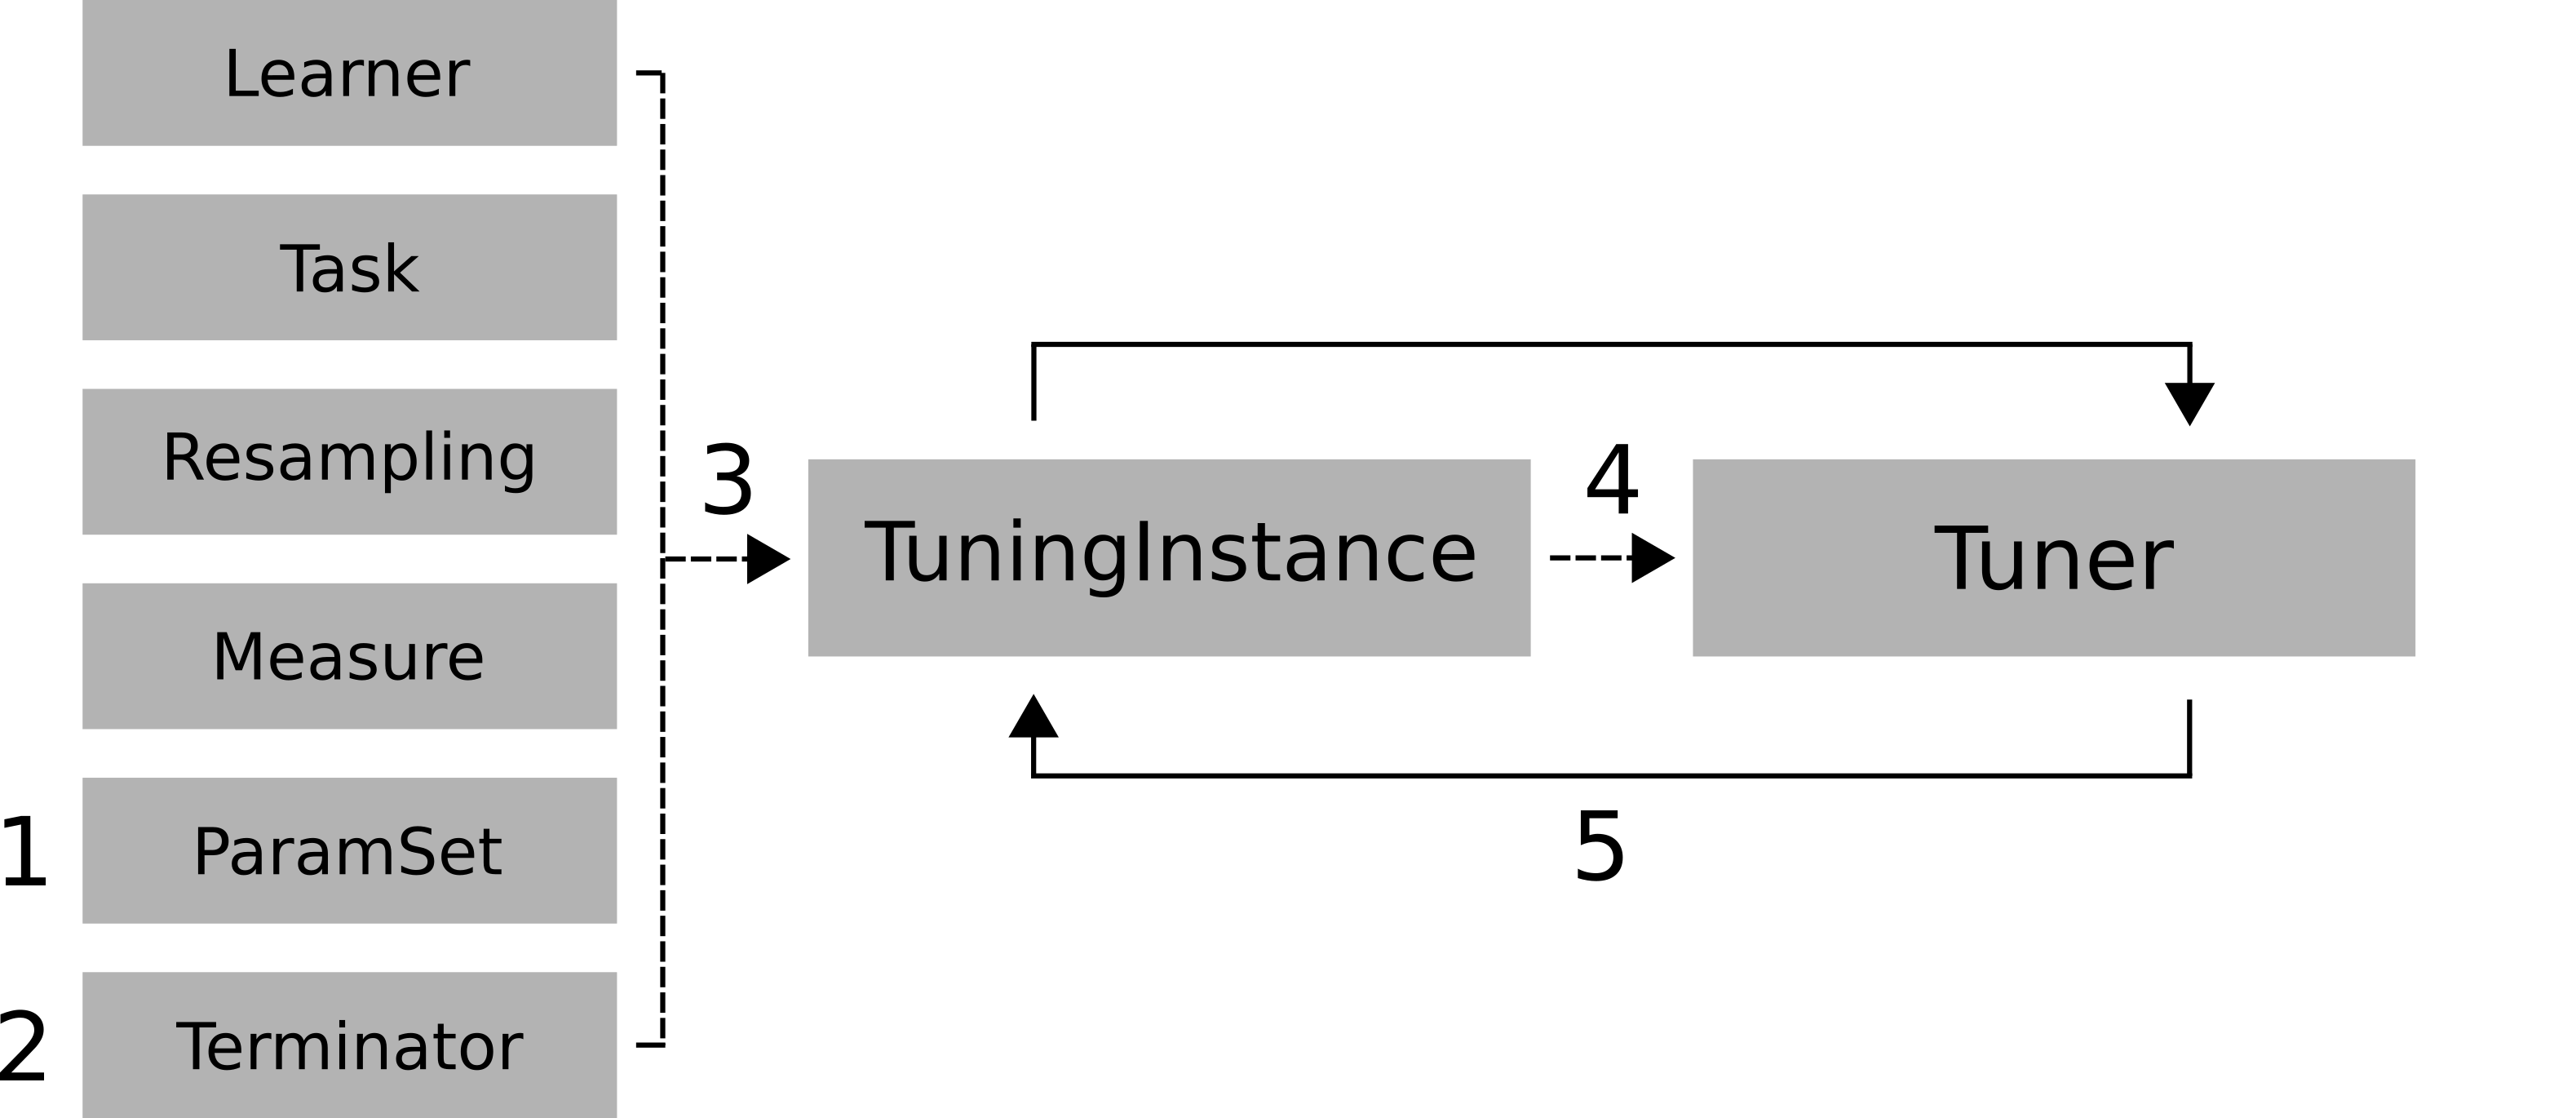
\includegraphics[width=\textwidth]{img/tuning_objects.png}
							% Main classes are \codeinline{TuningInstance} and \codeinline{Tuner}. 
						\end{myblock}
						\begin{myblock}{ParamSet}
					        Hyperparameters and ranges for tuning (1).
							\\
							\begin{codeboxmultiline}[width=21cm]
								tune\_ps = \textbf{ParamSet}\$new(list(\\
								\hspace*{1ex}\textbf{ParamInt}\$new(id, lower, upper),\\
								\hspace*{1ex}\textbf{ParamDbl}\$new(id, lower, upper),\\
								\hspace*{1ex}\textbf{ParamFct}\$new(id, levels),\\
								\hspace*{1ex}\textbf{ParamLgl}\$new(id)))
							\end{codeboxmultiline}
							% Constructs \codeinline{ParamSet} with different types of \codeinline{Param}s. 
                            Set \codeinline{id} to param id in the learner. Use \codeinline{lower} and \codeinline{upper} for numerical ranges, \codeinline{levels} for categories. 
                            % \codeinline{ParamFct} to define the factor levels to tune over.
							\\
							\begin{codebox}
								tune\_ps\$\textbf{add\_dep}(id, on, cond)
							\end{codebox}
							Adds dependency to the \codeinline{ParamSet}, so that \codeinline{id} depends on parameter \codeinline{on}.
							\codeinline{cond} is an object of class \codeinline{Condition}.
							\\
							\begin{codeboxmultiline}[width=26cm]
								tune\_ps\$\textbf{trafo} = function(x, param\_set) \{ \\
								\hspace*{1ex}x\$id = -log(x\$id)\}
							\end{codeboxmultiline}
							Set a transformation for parameter \codeinline{id}. 
							The function transforms the hyperparameter configuration into another encoding 
							before passing them to the \codeinline{Learner}.
						\end{myblock}
						\vfill}
				\end{minipage}
			\end{beamercolorbox}
		\end{column}
		\begin{column}{.245\textwidth}
			\begin{beamercolorbox}[center]{postercolumn}
				\begin{minipage}{.98\textwidth}
					\parbox[t][\columnheight]{\textwidth}{
						\begin{myblock}{Terminator}
							Stop criterion (2). Create with \codeinline{\textbf{term}(.key, ...)}
							\\
							\begin{itemize}
								\item \codeinline{clock\_time} 
								(\codeinline{secs}, \codeinline{stop\_time})\\
								After a given time.
								\item \codeinline{evals}
								(\codeinline{n\_evals})\\
								After a given amount of iterations.
								\item \codeinline{model\_time}
								(\codeinline{secs })\\
								After a given model time.
								\item \codeinline{perf\_reached}
								(\codeinline{level})\\
								After a specific performance.
								\item \codeinline{stagnation}
								(\codeinline{iters}, \codeinline{threshold})\\
								After the performance stagnates.
							\end{itemize}
							% \vspace{0.5cm}
							% Keys to access the \codeinline{Terminator} subclasses.
							% \\
							% \begin{codebox}
								% terminator = \textbf{term}(.key, ...)
							% \end{codebox}
							% Get terminator by \codeinline{.key} and construct terminator with settings (...) in one go.
							% \\
							\vspace{1.0cm}
							\begin{codebox}
								terminator = term("\textbf{combo}", terminators, any)
							\end{codebox}
							List of \codeinline{terminators} that terminate if any (\codeinline{any = TRUE}) or all (\codeinline{any = FALSE}) terminators are positive.
						\end{myblock}
						\begin{myblock}{TuningInstance}
							Defines search scenario. Evaluates configurations proposed by \codeinline{Tuner} and stores results. 
                            % (s. Triggering the tuning)(3).
							\\
							\begin{codeboxmultiline}[width=20cm]
								instance = \textbf{TuningInstance}\$new(\\
								\hspace*{1ex}task, learner, resampling,\\
								\hspace*{1ex}tune\_ps, terminator)
							\end{codeboxmultiline}
						\end{myblock}
						\vfill}
				\end{minipage}
			\end{beamercolorbox}
		\end{column}
		\begin{column}{.245\textwidth}
			\begin{beamercolorbox}[center]{postercolumn}
				\begin{minipage}{.98\textwidth}
					\parbox[t][\columnheight]{\textwidth}{
						\begin{myblock}{Tuner}
							% The \codeinline{Tuner} describes the tuning strategy. 
                            Tuning strategy. Create witth \codeinline{\textbf{tnr}(.key, ...)}
                            % and additionally hyperparameter configurations fully specified by the user:
							\\
							\begin{itemize}
								\item \codeinline{grid\_search}
								(\codeinline{resolution}, \codeinline{batch\_size})\\
								Grid search.
								\item \codeinline{random\_search}
								(\codeinline{batch\_size})\\
								Random search.
								\item \codeinline{gensa}
								(\codeinline{smooth}, \codeinline{temperature})\\
								Generalized simulated annealing.
								\item \codeinline{design\_points}
								(\codeinline{batch\_size }, \codeinline{design})\\
								All points user-specified.
							\end{itemize}
							\vspace{0.5cm}
							% Keys to access the \codeinline{Tuner} subclasses.
							% \\
							% \begin{codebox}
								% tuner = \textbf{tnr}(.key, ...)
							% \end{codebox}
							% Get the tuner by \codeinline{.key} and construct the tuner with settings (...) in one go.
						\end{myblock}
						\begin{myblock}{Start the tuning}
							% To start the tuning, \codeinline{TuningInstance} is passed to the \codeinline{\$tune} method of \codeinline{Tuner}.
							\begin{codebox}
								tuner\$\textbf{tune}(instance)
							\end{codebox}
							% Starts the tuning (4).
							%\\
							% \codeinline{Tuner} generates hyperparameter configurations and passes them to \codeinline{TuningInstance} until the budget of \codeinline{Terminator} is exhausted (5). To access the results: 
                            % use the following methods of \codeinline{TuningInstance}:
							% \\
                            To access the results: 
							\begin{codebox}
								instance\$\textbf{archive}(unnest)
							\end{codebox}
							Returns all tried configurations and their resampling results. Use \codeinline{unnest} to display hyperparameters without (\codeinline{tune\_x}) or with (\codeinline{params}) trafo applied.
							\\
							\begin{codebox}
								instance\$\textbf{result}
							\end{codebox}
							Returns list with optimal configuration and estimated performance.
							\\
							\begin{codeboxexample}
								\footnotesize{
									tune\_ps = ParamSet\$new(list(\\
									\hspace*{1ex} ParamDbl\$new("cp", lower = 0.001, upper = 0.1)))
									evals20 = term("evals", n\_evals = 20)
									\vspace{1em}
									\\
									instance = TuningInstance\$new(\\
									\hspace*{1ex} task, learner, resampling, measures,\\
									\hspace*{1ex} param\_set = tune\_ps, terminator = evals20)\\
									tuner = tnr("grid\_search", resolution = 5)
									\vspace{1em}
									\\
									tuner\$tune(instance)\\
									instance\$result
								}
							\end{codeboxexample}
						\end{myblock}
						\vfill}
				\end{minipage}
			\end{beamercolorbox}
		\end{column}
		\begin{column}{.245\textwidth}
			\begin{beamercolorbox}[center]{postercolumn}
				\begin{minipage}{.98\textwidth}
					\parbox[t][\columnheight]{\textwidth}{
						\begin{myblock}{Automatic Tuning}
							Wraps learner and adds automatic tuning. 
                            % for a given set of hyperparameters.
							\\
							\begin{codeboxmultiline}[width=20cm]
								at = \textbf{AutoTuner}\$new(\\
								\hspace*{1ex}learner, resampling, measures, \\
								\hspace*{1ex}tune\_ps, terminator, tuner)
							\end{codeboxmultiline}
							% Constructs the \codeinline{AutoTuner}.
							\vspace{1em}
                            Inherits from \codeinline{Learner} class; can be used like it. Training starts tuning on the training set, and after completion traisn the learner finally with this the optimal configuration on the full training set.
							% Automatic tuning is started by supplying \codeinline{task} to the \codeinline{\$train()} method.
							% \\
							% \begin{codebox}
								% at\$\textbf{train}(task)
							% \end{codebox}
							% The automatic tuning is started by supplying \codeinline{task} to the \codeinline{\$train()} method.
							% \\
							\begin{codeboxmultiline}
								at\$\textbf{train}(task)\\
								at\$\textbf{predict}(task, row\_ids)
							\end{codeboxmultiline}
							% Use the tuned \codeinline{Learner} in \codeinline{AutoTuner} to create a new \codeinline{Prediction} by supplying \codeinline{task} and \codeinline{row\_ids}.
							% \\
						\end{myblock}
						\begin{myblock}{Nested Resampling}
							In order to get unbiased performance estimates, 
							\{mlr3\} supports nested resampling for complex operations such as tuning.
							This can be achieved by passing a \codeinline{Resampling} strategy to
							\codeinline{resample()} as an outer resampling instance and using the 
							\codeinline{Resampling} strategy in \codeinline{AutoTuner} as an 
							inner resampling instance.
							\\
							\begin{codeboxmultiline}[width=26.5cm]
								resampling\_outer = rsmp("cv", folds = 3)
								rr = resample(task, \textbf{at}, \textbf{resampling\_outer})
							\end{codeboxmultiline}
							\vspace{1em}
							\begin{codebox}
								rr\$\textbf{aggregate()}
							\end{codebox}
							Aggregates performance results.
						\end{myblock}
						\vfill}
				\end{minipage}
			\end{beamercolorbox}
		\end{column}
	\end{columns}
\end{frame}
\end{document}
